\chapter{Benchmark orodja in platforma Azure}

\pagestyle{fancy}
\fancyhf{}
\fancyhead[LE,RO]{\thepage}
\fancyhead[RE,LO]{\leftmark}

\huge Žiga Šebenik, Tomaž Mrežar


\normalsize
\bigskip

\section{Opis problema}
Za določanje zmogljivosti računalniških sistemov je na voljo veliko orodij, tako odprtokodnih, zastonjskih kot tudi plačljivih. V tem poglavju bomo predstavili orodja in postopke, s katerimi smo testirali virtualni računalnik na Microsoftovem oblaku Azure, kjer smo imeli odprt brezplačni račun. Na njem smo pognali različna bremena, kjer smo testirali omrežne povezave, diskovje in procesor. Nekaj od teh bremen smo ustvarili s pomočjo zastonjskih programov: Geekbench 3 za test procesorja, iPerf za test omrežja, ioPing za latenco diskovja in fio za test pasovne širine diskovja. Vsako orodje smo opisali in našteli prepoznavne značilnosti in prednosti pred ostalimi orodji. Ostala bremena smo ustvarili sami. Napisali smo namreč dva kratka programa, enega za test omrežja in diska hkrati, ter enega za test moči procesorja. Ta dva programa smo pognali na naših računalnikih, prav tako pa smo jih pognali tudi na virtualnem računalniku, da smo lahko primerjali zmogljivosti. Računalnika se razlikujeta v moči, saj je en računalnik prenosnik, drugi pa osebni računalnik, razlika pa je tudi v lokaciji, saj smo teste poganjali iz Kranja in Brezovice pri Ljubljani. Imava tudi različna ponudnika interneta, kar vse pride v poštev pri testih. Iz rezultatov testiranja smo nato poskušali sklepati o razlogih za razlike, ki so se pri teh testih pojavile.
  
\begin{figure}[H]
	\centering
	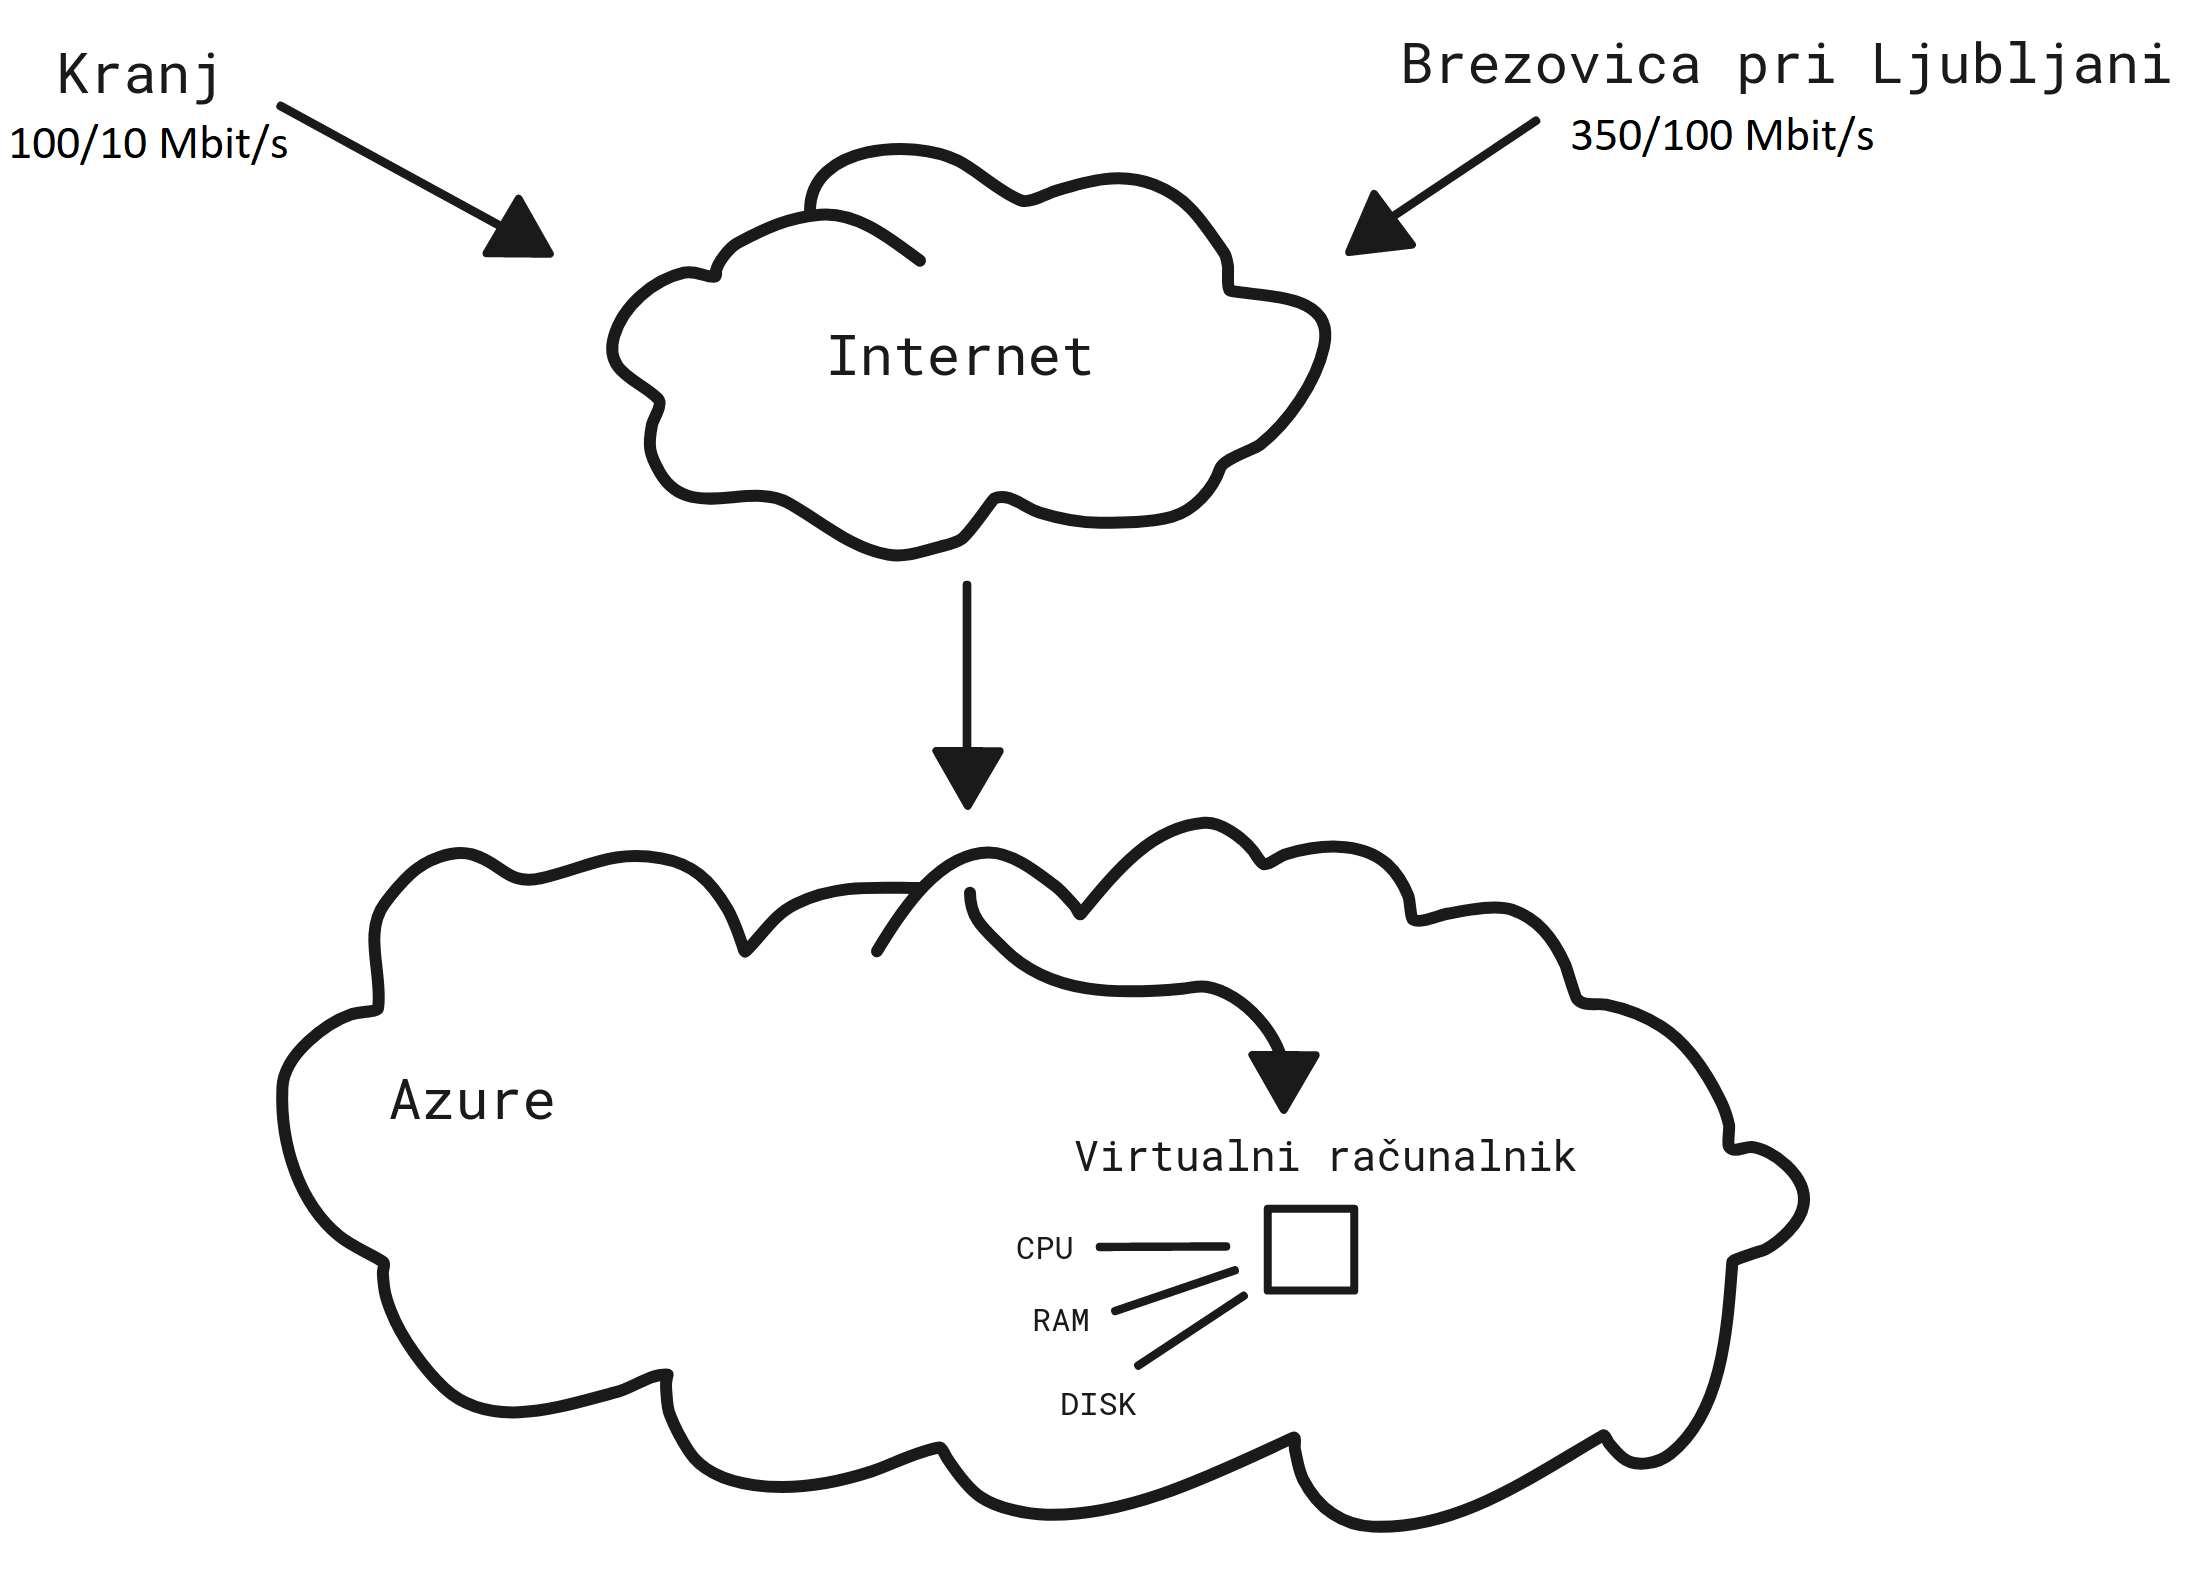
\includegraphics[scale=0.15]{Img/3_celotni_diagram.png}
	\caption{Celotni prikaz testiranja na Azure platformi.}
	\label{fig:3_7_breme2}
\end{figure}


\section{Benchmark orodja}
Obstaja več vrst benchmark orodij. Testi, ki jih benchmark orodja izvajajo se lahko razlikujejo med seboj vendar so osnovne funkcionalnosti testov skoraj povsod enake. Skorajda vsako orodje testira dosegljivost sistemov, upočasnitve delovanja, latenco sistema in prepustnost sistema. Orodja bomo delili na dve skupini, prva skupina bodo orodja, ki so brezplačna, medtem ko bodo v drugo skupino spadala orodja, ki so plačljiva, brezplačna za določen čas ali pa imajo v brezplačni verziji omejene funkcionalnosti.

\section{Brezplačna orodja}
Brezplačni orodji sta sledeči:
\begin{itemize}
\item ročno benchmark testiranje;
\item PerfKit Benchmarker;
\end{itemize}

\subsection{Ročno benchmark testiranje}
Zelo preprosta izbira, ki nam je na voljo, je da preprosto sami testiramo zmogljivost oblačnih storitev s pomočjo več različnih orodij,pri čemer je vsako namenjeno specifičnemu delu sistema. Na voljo nam je veliko zastonjskih orodij, precej jih je tudi odprtokodnih, znani med njimi pa so ping, Geekbench, fio, iPerf... Testiramo lahko zmogljivost posameznega strežnika, gruče ali pa celotnega oblaka. Njihova prednost je, da so preprosta in fleksibilna, vendar pa moramo več dela opraviti sami.

\subsection{PerfKit Benchmarker}
PerfKit Benchmarker je odprtokodno orodje uporabljeno za meritve in primerjave oblačnih performans.
Podpira več večjih oblačnih ponudnikov, kot sta Google Cloud Platform in Amazon Web Services, pa tudi mnoge druge.
PerfKit Benchmarker meri končni čas za zagotavljanje virov v oblaku in tudi vse osnovne oblačne meritve naštete v predhodnem razdelku. PerfKit Benchmarker zmanjšuje kompleksnost v zaganjanju testov na oblačnih ponudnikih z enotnimi in preprostimi ukazi.
Vsebuje tudi množice javnih testov za uporabo. Vsi testi se zaženejo z privzeto konfiguracijo, ki ni nastavljena v prid nobenemu ponudniku oblačnih storitev. To ponuja možnost testiranja na več različnih oblačnih platformah.
V bistvu je Perfkit Benchmarker le orodje, ki avtomatizira zagon ostalih, ozko nameskih orodij za test posameznih metrik platforme. Vsa orodja, ki jih uporablja so odprtokodna in bi jih lahko pognali sami, vendar nam Perfkit Benchmarker, zmanjša količino dela, saj ima prilagojene skripte za vse večje ponudnike.

\section{Plačljiva orodja}
Plačljiva orodja so sledeča:
\begin{itemize}
\item SPEC Cloud® IaaS 2018;
\item Cloud Spectator;
\item Cloud Performance Benchmark;
\item Technology Business Research, Inc.;
\end{itemize}

\subsection{SPEC Cloud® IaaS 2018}

SPEC Cloud® IaaS 2018 testira delovanje infrastrukture kot storitev oblačnih implementacij \cite{SPEC}. Podpira testiranje javnih in zasebnih oblakov. Orodje deluje nad strežbo storitve, kot tudi nad izvajanjem storitve oblaka z uporabo vhodno izhodnih in CPE intenzivnih del. Vsako delo se zažene kot distribuirana aplikacija narejena iz 6 ali 7 instanc, ki obremenijo oblakove resource (CPE, diski in omrežje). Delo bo teklo dokler testi ne naredijo več kakovosti storitve. Administrator lahko tudi omeji število aplikacij kreiranih med izvedbo.
Orodje nam omogoča obremeniti računsko zmogljivost, shrambo in omrežje oblaka. Pri tem pa ne potrebuje hypervizorja ali virtualizacijske plasti in uporablja delovne obremenitve, ki spominjajo na tiste, ki običajno delujejo v oblaku, kot so aplikacije za socialne medije in velika analiza podatkov.
SPEC Cloud izdaja poročila, ki ne grejo tako v detajle posameznega dela platforme ter izdajajo ločene metrike za vsak del platforme, ampak testirajo zmogljivost ponudnikove platforme kot celote. Merijo čas stvaritve, konfiguracije in zagona instanc oz. virtualnih strojev, latenco vstavitve oz. branja iz baze na postavljeni virtualki, prepustnost, skalabilnost. Vse metrike so merjene v sekundah oz. operacijah na sekundo.

\subsection{Cloud Spectator}

Cloud Spectator sicer ni orodje, ampak podjetje, ki ponuja benchmarking in konzultacijo glede oblačnih storitev \cite{cloudSpectator}. Podjetjem pomaga z analizo različnih ponudnikov oblačnih storitev in testira zmogljivost njihove infrastrukture ter svetuje pri ekonomskih odločitvah. Namenjen je tako primerjavi ponudnikov oblačnih storitev, kot tudi ponudnikom samim, da lahko analizirajo zmogljivost svoje infrastrukture. Nudili naj bi sposobnost izbire pravega ponudnika, kjer stranka postavi zahteve svoje aplikacije, Cloud spectator pa s kombinacijo zahtevosti strankine aplikacije, zmogljivosti infrastrukture različnih ponudnikov in njihovih cenikov, izbere pravega ponudnika.
Poročilo vrača rezultate v obliki VM Performance Sore in CloudSpecs Score. Nobeden od njiju nima posebne merske enote, saj je VM Performance Score le povprečje točk, ki jih vrneta Geekbench 4 in fio, tako da imata oba enak prispevek k točkam. CloudSpecs Score se izračuna kot VM Performance Score, ki je utežen s ceno, tako da dobimo zmogljivost na ceno, ki naj bi strankam omogočala lažjo izbiro pravega ponudnika platforme.

\subsection{Cloud Performance Benchmark}

Cloud Performance Benchmark je poročilo o največjih petih ponudnikih Amazon Web Services, Google Cloud Platform, Microsoft Azure, IBM Cloud in Alibaba Cloud \cite{thousandEyes}. Zagotavljalo naj bi nepristransko strokovno poročilo, ki je podprto z raznimi metrikami. Poročilo primerja infrastrukturo posameznega ponudnika in pokaže kako ta infrastruktura vpliva na zmogljivost ter jih seveda primerja med seboj. Prav tako se dotakne geografskih razlik in njihov vpliv na zmogljivost.
Poročilo ne vsebuje le kvantitativnih podatkov o posameznih platformah, temveč tudi veliko več kvantitativnih in statističnih podatkov o predvidljivosti posameznih metrik poleg razlag arhitektur vsake platforme. Poročilo je zelo poglobljeno, kvantitativne metrike pa se tičejo predvsem omrežja, saj je velik poudarek na latenci, tako izven kot znotraj platforme, ter izgubi paketov. Veliko podatkov najdemo tudi o vplivu geografskih pozicij na kakovost omrežja vsake platforme, vse podprto z statistično analizo obeh metrik.

\subsection{Technology Business Research, Inc.}

Technology Business Research, Inc. je podjetje, ki prav tako nudi storitve tako ponudnikom oblačnih storitev, kot tudi njihovim strankam 
\cite{TBR}. Ponudnikom nudijo podatke o trgu, finančne podatke o ponudnikih programske opreme, napovedi, strategije prodaje, itd. Ponudnikom oblačnih storitev pa nudijo podatke o ponudnikih le teh storitev, zmogljivosti ponudnikove infrastrukture za strankin primer uporabe ter tudi prihajajoče trende, ki se bodo posluževali in vplivali na zmogljivost oblačnih sistemov.
TBR Inc. je bolj usmerjeno v svetovanje situaciji na trgu, kot pa poglobljeni analizi metrik in zmogljivosti. Sledijo trendom in priložnostim na trgu, napovedujejo nove trende in sledijo finančnim podatkov ponudnikov platform. Njihov glavni cilj je direktni stik in osebno svetovanje strankam, zato nismo uspeli najti nobenih uporabnih podatkov o njihovi metodologiji oz. metrikah.


\section{Implementacija merilnega okolja}
Na oblaku Microsoft Azure smo ustvarili račun in na njem postavili virtualni stroj, ki poganja Ubuntu 18.04. Na tej virtualki smo ročno pognala več benchmark testov, saj googlov odprtokodni Perfkit Benchmarker ni deloval. Le ta se namreč zanaša na avtomatsko ustvarjanje virtualnih strojev, zastonjski račun na Azure pa to omejuje. Pognali smo odprtokodna orodja:
\begin{itemize}
\item Geekbench 3 = uporabljen predvsem za test CPE zmogljivosti;
\item  test pasovne širine omrežja in dostop do interneta;
\item  latenca diskovja;
\item  zmogljivost diskovja;
\end{itemize}

\subsection{Tehnične specifikacije računalnika}
Specifikacije računalnika na katerem teče virtualni stroj so sledeče:

\begin{itemize}
\item OS: Ubuntu 18.04.4 LTS 5.0.0-1032-azure x86\_64
\item CPE: Intel Xeon Platinum 8168 @ 2.69 GHz 1 processor, 2 threads
\item RAM: 4 GB
\item Disk: 32 GB SSD
\end{itemize}
Ker se računalnik nahaja nekje v Microsoftovem strežniškem centru in ker uporabljamo zastonjski račun na Azure, nimamo na razpolago celotnega računalnika, saj na njem verjetno teče tudi kakšna druga virtualka, kar zna vplivati na rezultate meritev. Omenjene specifikacije računalnika so le te, ki jih imamo na voljo na virtualki. Lokacija strežnika je Nizozemska.


\section{Rezultati meritev}

V naslednjih razdelkih bomo predstavili testna orodja uporabljena na virtualnem računalniku in dobljene rezultate.

\subsection{Geekbench 3}
Najprej smo pognali Geekbench 3, benchmark, ki se uporablja za testiranje CPE zmogljivosti. Imel naj bi to prednost pred klasičnimi testi CPE, da simulira tako breme na procesorju, ki dobro ponazarja produkcijsko okolje med izvajanjem realnih programov, in ne samo sintetično breme. Prav tako Geekbench dodobra obremeni računalnik, da lahko vidimo zmogljivost ob velikem stresu. Še ena dobra stvar kar se tiče Geekbench-a je, da je zelo razširjen, kar pomeni da lahko najdemo veliko različnih rezultatov testov za različne konfiguracije računalnikov, vendar pa to ne pomeni da je zanesljiv. Obstajajo namreč primeri, kjer ima strežniški CPE slabšo oceno kot nek mobilni CPE, saj Geekbench ne testira termalnih zmogljivosti, prav tako pa so razlike med rezultati na različnih operacijskih sistemih. Čeprav Geekbench uporabi več različnih testov, iz povzetka vseh teh testov vrne dve glavni številki: Single-core točke in Multi-core točke, ki sami po sebi nič ne pomenita in nimata merskih enot, velja pa višje je, bolje je. Šele ko ju primerjamo z ostalimi sistemi, dobimo neko sliko zmogljivosti. 

Na sliki \ref{fig:3_1_geekbench1} so predstavljeni rezultati večih algoritmov za performanse celih števil. Algoritmi se izvajajo na enem jedru procesorja in na večih.
\begin{figure}[H]
    \centering
    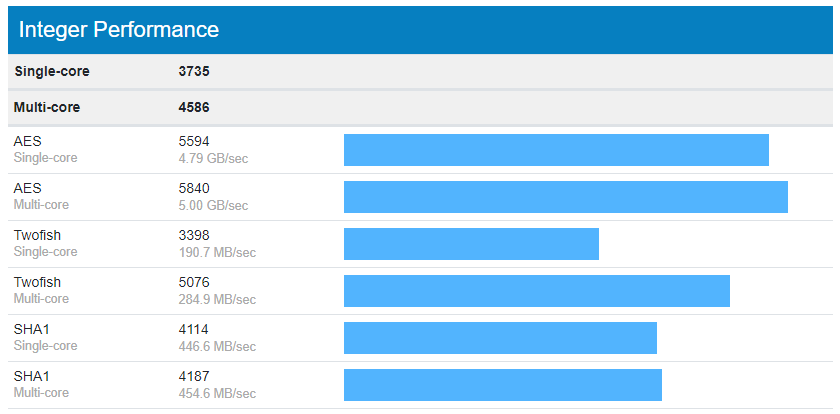
\includegraphics[scale=0.5]{Img/3_geekbench1.png}
    \caption{Cela števila.}
    \label{fig:3_1_geekbench1}
\end{figure} Na sliki \ref{fig:3_2_geekbench2} so predstavljeni rezultati večih algoritmov za performanse števil v plavajoči vejici. Algoritmi se izvajajo na enem jedru procesorja in na večih.
\begin{figure}[H]
    \centering
    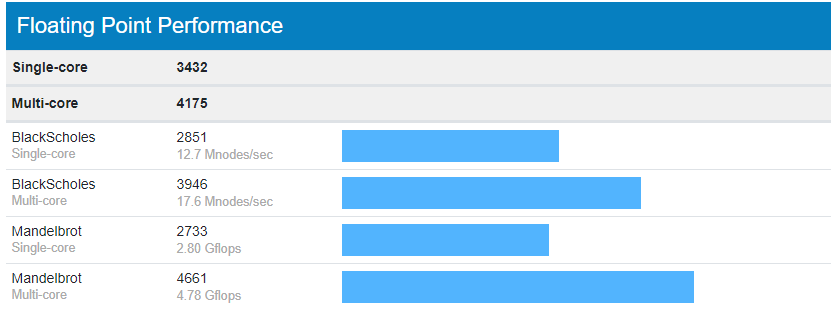
\includegraphics[scale=0.5]{Img/3_geekbench2.png}
    \caption{Plavajoča vejica.}
    \label{fig:3_2_geekbench2}
\end{figure} Na sliki \ref{fig:3_3_geekbench3} so predstavljeni rezultati za testiranje spomina. Testira se z kopiranjem na večih jedrih in na enem jedru procesorja.
\begin{figure}[H]
    \centering
    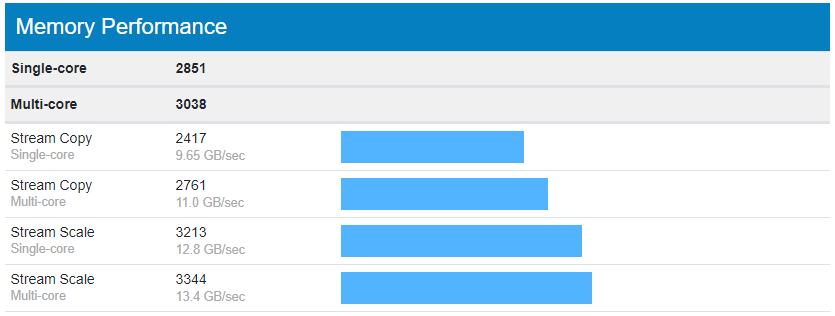
\includegraphics[scale=0.5]{Img/3_geekbench3.png}
    \caption{Performanse spomina.}
    \label{fig:3_3_geekbench3}
\end{figure}

\subsection{iPerf}
Naslednji benchmark, ki smo ga pognali je iperf, ki meri podatke o omrežju kot sta upload in download pasovno širino. Meri jih v enotah bajt/sekunda, kjer prilagodi prefix od bajta glede na hitrost omrežja. Test smo pognala nad omrežjem med nami in virtualnim strojem. Čeprav bi lahko v našem primeru podatke popačila hitrost ponudnika interneta na naši strani, pa temu verjetno ni tako, saj smo testirali na omrežju z 12 MB/s prenosa. Nismo prepričani, ali isto velja tudi za upload hitrost, latence pa nismo testirali, saj se strežnik nahaja na nizozemskem in latenca zaradi geografske lokacije pač je kakršna je. Iperf nam vrne povprečno hitrost prenosa podatkov 2,71 MB/s in 2,53 hitrost uploada podatkov, kjer velja, da večje številke pomenijo boljše performanse. Na sliki \ref{fig:3_4_iperf1} so predstavljeni rezultati testa iPerf, kjer lahko vidimo hitrosti prenosa na intervalih.
\begin{figure}[H]
    \centering
    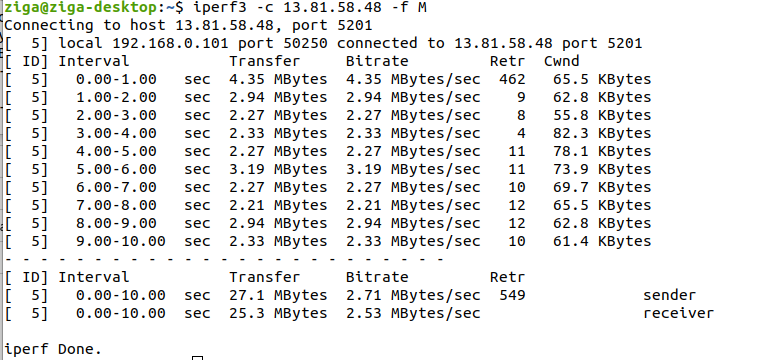
\includegraphics[scale=0.5]{Img/3_iperf1.png}
    \caption{test iPerf.}
    \label{fig:3_4_iperf1}
\end{figure}


\subsection{ioPing}
Tretji benchmark, ki smo ga izbrali je ioPing. Prednost ioPing-a naj bi bila njegova preprostost, saj je zelo podoben znanemu ukazu ping, le da je namenjen testu diskovja v računalniku. Ni namenjen testiranju diskovja pod naporom, zanima ga le latenca zahtev za pisanje/branje. Le ta je izredno pomembna za podatkovne baze, ki niso pod velikim stresom zaradi števila zahtev, vendar bi njihov opazen zamik pri odzivu negativno vplival na uporabniško izkušnjo. Latenca nima velikega pomena pri večih asinhronih operacijah pisanja, saj je to veliko bolj odvisno od prepustnosti diska. Zato smo pognali testa latence pri sinhronih oz. zaporednih operacijah pisanja in latenci pri asinhronih operacijah branja. ioPing poda rezultate latence v obliki sekund, seveda pa prilagodi predpono velikosti latence. SSD, do katerega dostopa virtualka, je precej hiter in ima latenco v rangu 200 mikrosekund, kjer sta pomembni še minimum in maksimum vrednosti latence. Standardni odklon (mdev) nam pove kakšen razpon latenc lahko pričakujemo pri večini operacij. Na sliki \ref{fig:3_5_ioping1} so predstavljeni rezultati testa ioPing, kjer lahko vidimo odzivne čase.
\begin{figure}[H]
    \centering
    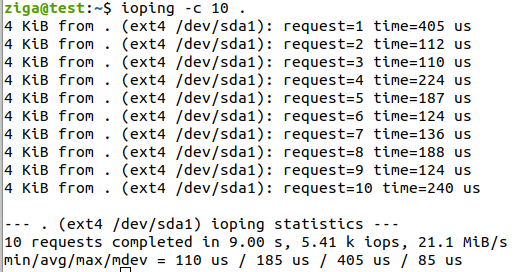
\includegraphics[scale=0.5]{Img/3_ioping1.png}
    \caption{test ioPing.}
    \label{fig:3_5_ioping1}
\end{figure}

\subsection{Fio}
Četrti benchmark, ki smo ga pognali je program fio, kar pomeni "flexible I/O". Fio je precej fleksibilen in torej bolj kompleksen program za testiranje diskovja, omogoča več specifičnih testov. Uporabljajo ga razvijalci in administratorji, za testiranje delovanje diskovja in datotečnih sistemov. Mi smo ga uporabili za test pasovne širine pisanja/branja, samo pisanja ali samo branja na disk. V povprečju neka standardna podatkovna baza dobi 3 bralne operacije za vsako pisalno operacijo, torej je razmerje med read in write operacijami 3:1. To razmerje smo uporabili pri testu kombinacije pisanja in branja. Na sliki \ref{fig:3_6_fio1} so predstavljeni rezultati testa Fio za read in write, kjer smo ukaz za zagon testa našli na 
spletni strani programmer.help. \cite{proghelpFio}
\begin{figure}[H]
    \centering
    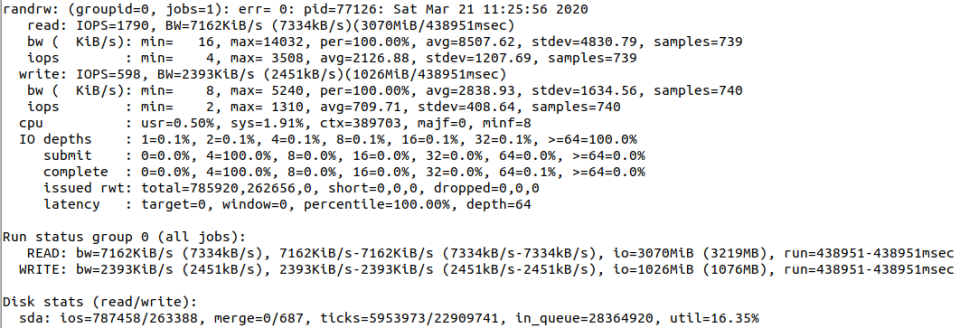
\includegraphics[scale=0.4]{Img/3_fio1.png}
    \caption{test Fio, R/W.}
    \label{fig:3_6_fio1}
\end{figure}

\subsection{Lastnosti metrik testov}

Tabela prikazuje metrike uporabljenih testov. Njihove slabosti in prednosti pred drugimi.

\begin{table}[H]
    \centering
        \begin{tabular}{ | r | r | r | r | r |} 
            \hline
            Metrike & Geekbench 3 & iPerf & ioPing & Fio  \\
            \hline
            linearnost & NE & DA & NE & NE \\
            zanesljivost & NE & DA & NE & DA  \\
            ponovljivost & DA & NE & DA & NE  \\
            enostavnost & NE & DA & DA & DA  \\
            konsistentnost & DA & DA & NE & DA  \\
            neodvisnost & NE & DA & DA & DA  \\
            \hline
        \end{tabular}
        \caption{Metrike  testov.}
    \label{table:1_chunks}
\end{table}



\section{Zmogljivost omrežnih povezav}

Merjenje zmogljivosti povezav do virtualnega računalnika smo izmerili z uporabo orodja PING in Traceroute.

\subsection{RTT}
Pri naslednjih razdelki se bo uporabljala beseda RTT, katero bomo definirali tukaj. RTT (angl. Round Trip Time) ali po slovensko čas povratnega potovanja. Z besedo opišemo čas, ki je potreben za pošiljanje in prihod paketa do destinacije + čas potovanja potrditve do izvora.

\subsection{Ping}
Ping je administracijsko programsko orodje, katerega se uporablja za testiranje dosegljivosti in latence nekega omrežja preko IP protokola. Ping meri RTT sporočil poslanih od izvora do destinacije. Deluje na protokolu ICMP, kateri pošlje zahtevo in počaka na odziv.

\subsection{TraceRoute}
TraceRoute je orodje, ki se uporablja za prikaz poti od izvora do destinacije preko protokola IP. Zgodovina skokov paketa je shranjena kot RTT paketov prejetih od vsakega naslednjega vozlišča. Vsota povprečnih časov vsakega skoka je meritev celotnega časa potrebnega za vzpostavitev povezave.

\subsection{Implementacija}
Na virtualnem računalniku je bilo potrebno nastaviti pravilo, da se računalnik odziva na ICMP pakete katere prejme. Neodzivanje na ICMP pakete se lepo vidi iz slike \ref{fig:3_6_traceroute1}, kjer * predstavljajo vse usmerjevalnike na poti kateri se niso odzvali. Na sliki \ref{fig:3_6_traceroute1} se vidi testiranje iz lokacije Kranja, medtem ko na sliki \ref{fig:3_6_traceroute2} lahko vidimo testiranje iz lokacije Brezovica pri Ljubljani. Virtualni računalnik se nahaja na Nizozemskem, zato je zadnjih nekaj skokov skoraj enakih, razlikujejo se le v številkah serverja, skozi katerega so paketi potovali. Na lokaciji Brezovica pri Ljubljani je prihodna/odhodna hitrost 100/10, na 
lokaciji Kranj pa 50/5. 

\begin{figure}[H]
    \centering
    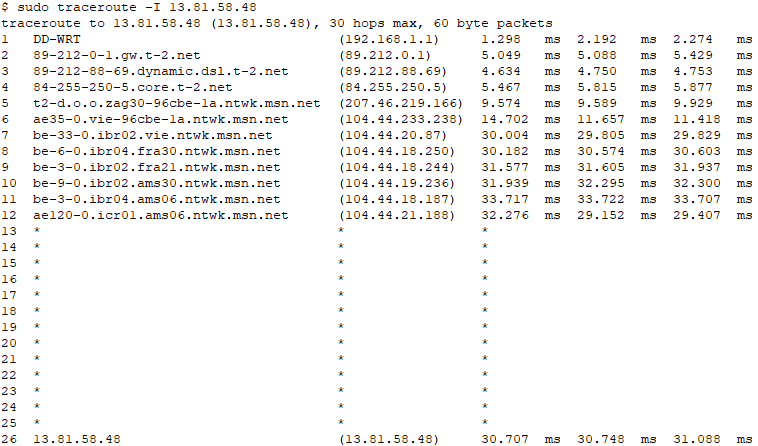
\includegraphics[scale=0.45]{Img/3_traceroute1.png}
    \caption{Prikaz poti iz Kranja do virtualnega računalnika.}
    \label{fig:3_6_traceroute1}
\end{figure}

\begin{figure}[H]
    \centering
    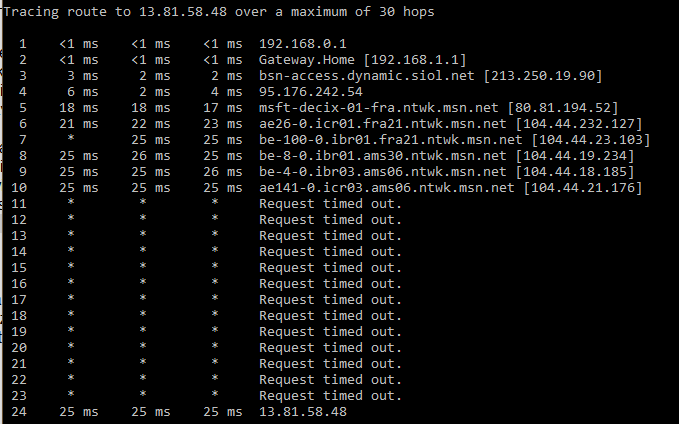
\includegraphics[scale=0.5]{Img/3_traceroute2.png}
    \caption{Prikaz poti iz Brezovice pri Ljubljani do virtualnega računalnika.}
    \label{fig:3_6_traceroute2}
\end{figure}


\subsection{Umetno breme}

Za bolj podrobno testiranje omrežja smo pripravili 2 programa. Prvi program iz lokalnega računalnika pošilja datoteko poljubne velikosti, v tem programu lahko tudi določimo interval pošiljanja datoteke. Za ustvarjanje datoteke poljubne velikost smo si pomagali z ukazom na spletni strani skorks.com \cite{skorks}. Drugi program pa je treba pognati na našem virtualnem računalniku na katerem sprejema datoteko in po uspešnem sprejemu pošlje čas prejetja, katerega prvi program izpiše.
Cilj programov je testirati hitrost procesiranja datoteke brez zapisovanja na disk.
Na sliki \ref{fig:3_7_breme1} lahko vidimo čase pošiljanja na 5 sekund z zelo malo nihanja. Zelo malo nihanja je zato, ker ima virtualni računalnik, ki prejema datoteke dovolj časa, da stvari procesira. 

\begin{figure}[H]
    \centering
    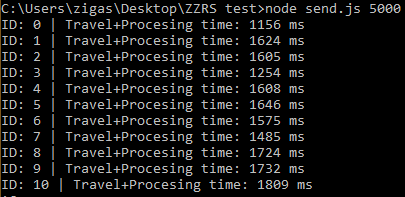
\includegraphics[scale=0.8]{Img/3_breme1.png}
    \caption{Časi pošiljanja na 5 sekund.}
    \label{fig:3_7_breme1}
\end{figure}

Če zmanjšamo interval pošiljanja na 0.5 sekunde se časi povečajo, saj virtualni računalnik nima dovolj hitrega procesiranja datotek in zaradi tega prihaja do zamud. To lahko vidimo tudi na sliki \ref{fig:3_7_breme2}, kjer se je čas prejemanja iz povprečno 1.2 sekunde povečal na povprečno 7 sekund.

\begin{figure}[H]
    \centering
    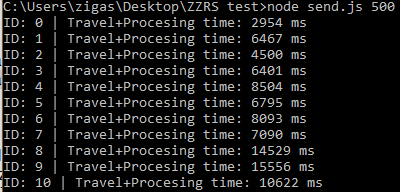
\includegraphics[scale=0.8]{Img/3_breme2.png}
    \caption{Časi pošiljanja na 0.5 sekunde.}
    \label{fig:3_7_breme2}
\end{figure}

Na zadnji sliki \ref{fig:3_7_breme3} lahko vidimo, da je idealen čas pošiljanja datotek na približno 900 milisekund ali 0.9 sekunde. Idealen je zaradi tega, ker se datoteke pošiljajo z najhitrejšim intervalom z majhnim povprečnim časom.

\begin{figure}[H]
    \centering
    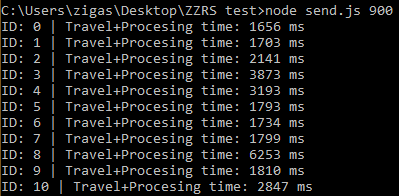
\includegraphics[scale=0.8]{Img/3_breme3.png}
    \caption{Časi pošiljanja na 0.9 sekunde.}
    \label{fig:3_7_breme3}
\end{figure}

\section{Zmogljivost diskovnega sistema}

Po sprejemu datoteke od pošiljatelja, sprejemnik pošlje svoj odgovor, datoteka pa ostane le v pomnilniku in se ne zapiše na disk. Da bi testirali tudi hitrost pisanja datotek na disk, smo ustvarili več datotek različnih velikosti, vsako od njih večkrat poslali na virtualni računalnik, ter jo po sprejetju tudi zapisali na disk. Merili smo čas od začetka zapisovanja do konca zapisovanja vsake datoteke, potrebno pa je upoštevati, da je disk, ki ga ima virtualni računalnik na voljo, precej hiter SSD.

\begin{table}[H]
	\centering
	\begin{tabular}{ | r | r | r | r | }
		\hline
		Čas pošiljanja & Min [ms] & Povprečje [ms] & Max [ms]  \\
		\hline
		1 MB & 1751 & 2273 & 2945 \\
		2 MB & 3377 & 3830 & 4589 \\
		5 MB & 3918 & 4012 & 4277 \\
		10 MB & 8208 & 8356 & 8532 \\
		20 MB & 17019 & 17160 & 17371 \\
		40 MB & 34819 & 35094 & 35439 \\
		\hline
	\end{tabular}
	\caption{Metrike  testov.}
	\label{table:1_chunks}
\end{table}

Najprej smo za vsako prejeto datoteko v pomnilniku na virtualnem računalniku ustvarili novo datoteko na disku. Povprečni časi zapisovanja so precej nizki zaradi SSD diska, odstopanja pa so razmeroma velika.

\begin{table}[H]
	\centering
	\begin{tabular}{ | r | r | r | r | }
		\hline
		Čas shranjevanja & Min [ms] & Povprečje [ms] & Max [ms]  \\
		\hline
		1 MB & 1 & 1.3 & 4 \\
		2 MB & 1 & 1.73 & 2 \\
		5 MB & 3 & 3.36 & 4 \\
		10 MB & 6 & 6.8 & 8 \\
		20 MB & 12 & 14.7 & 22 \\
		40 MB & 27 & 30.3 & 34 \\
		\hline
	\end{tabular}
	\caption{Metrike  testov.}
	\label{table:1_chunks}
\end{table}

Zanimivi so rezultati, ki smo jih dobili, ko smo vsako prejeto datoteko v pomnilniku zapisali v isto datoteko na disku. Seveda smo prepisali vsebino prejšnje prejete datoteke. Povprečni čas se je namreč močno podaljšal, minimum pa je ostal podoben prejšnjemu. Ni nam povsem jasno, zakaj se to zgodi, vendar je odstopanje od pisanja vsakič v novo datoteko preveliko, da bi ga lahko zanemarili.

\begin{table}[H]
	\centering
	\begin{tabular}{ | r | r | r | r | }
		\hline
		Čas shranjevanja & Min [ms] & Povprečje [ms] & Max [ms]  \\
		\hline
		1 MB & 1 & 1.3 & 2 \\
		2 MB & 2 & 2.3 & 5 \\
		5 MB & 4 & 24.6 & 91 \\
		10 MB & 9 & 63.3 & 112 \\
		20 MB & 18 & 192.3 & 225 \\
		40 MB & 80 & 255.9 & 348 \\
		\hline
	\end{tabular}
	\caption{Metrike  testov.}
	\label{table:1_chunks}
\end{table}

\section{Zmogljivost procesorja}

V tem razdelku bomo testirali zmogljivost procesorja na virtualnem računalniku in na domačih lokacijah.


\subsection{Opis programa}

Program, ki bo testiral zmogljivost smo napisali sami, program deluje na enem jedru procesorja in ne uporablja diskovnih pogonov.
Osnovna naloga programa je, da z matematično intenzivnim problemom testira hitrost procesorja, za kar smo v našem programu pripravili dva taka problema. Oba problema uporabljata zelo malo dinamičnega pomnilnika in oba sta implementirana z algoritmoma, ki imata časovno zahtevnost O($n$). Vsak algoritem se kliče večkrat, zaradi tega je časovna zahtevnost celotnega programa O($n$\textsuperscript{2}). Ko se program zaključi se izpiše čas izvajanja enega in drugega algoritma, nato pa izpiše še skupni čas izvajanja obeh problemov.



\subsection{Algoritem za faktorizacijo}

Prvi algoritem za vsa števila na intervalu [10.050.000, 10.050.500] izračuna faktoriteto (npr. 5! = 120). Algoritem ne uporablja nobenih izblojšav s katerimi se lahko pohitri njegovo delovanje. Implementacijo algoritma lahko vidite v izpisu \ref{3_lst:alg1}.

\begin{lstlisting}[language=C++, caption=Algoritem računanja faktoritele, label={3_lst:alg1},captionpos=b]
void factorialTEST()
{
    long N = 10050000;

    long iterations = 500;

	for(int i=0;i<iterations;i++)
	{
		long c, n = N, f = 1;
		for (c = 1; c <= n; c++)
			f = f * c;

		n++;
	}
}
\end{lstlisting} 

Algoritem za faktorizacijo naredi 500 ponovitev. Pri vsaki ponovitvi se naredi \textit{N+1} primerjav, \textit{C+2} seštevanj in \textit{N} množenj. Začetno število \textit{N} za izračun faktoritete je 10.050.000. Število za izračun se pri vsaki ponovitvi poveča za 1. Algoritem uporablja podatkovne strukture tipa long, kar je pri vseh računalnikih na katerih se je testiral 64-bitov. 

\subsection{Algoritem za iskanje praštevil}

Drugi algoritem za vsa števila na intervalu [10.050.000, 10.055.000], preveri če je število praštevilo. Algoritem ne uporablja nobenih izblojšav, s katerimi se lahko pohitri njegovo delovanje. Implementacijo algoritma lahko vidite na izpisu \ref{3_lst:alg2}.

\begin{lstlisting}[language=C++, caption=Algoritem za iskanje praštevil, label={3_lst:alg2},captionpos=b]
bool isPrime(int n)
{
    if (n <= 1)
        return false;

    for (int i = 2; i < n; i++)
        if (n \% i == 0)
            return false;

    return true;
}


void primeTEST()
{
	long N = 10050000;

	long iterations = 5000;

	for(int i=N;i<N+iterations;i++)
	{
		isPrime(i);
	}
}
\end{lstlisting} 


Algoritem za preverbo praštevil naredi 5000 ponovitev. Pri vsaki ponovitvi se naredi v najslabšem primeru \textit{N} primerjav, \textit{N+1} seštevanj in \textit{N} deljenj. Začetno število \textit{N} za preverbo pripadnosti praštevilom je 10.050.000. Število za izračun se pri vsaki ponovitvi poveča za 1. Algoritem uporablja podatkovne strukture tipa long in int, kar je pri vseh računalnikih, na katerih se je testiral za tip long 64-bitov za tip int pa 32-bitov. 



\subsection{Rezultati meritev}

Program smo pognali tako na naših računalnikih, na prenosnem in osebnem računalniku, kot seveda tudi na virtualnem računalniku na Azure platformi. Ročno smo za vsak slučaj preverili, da program uporablja dejansko samo eno CPU jedro, malo pomnilnika in ne piše na disk, kar smo storili z uporabo sistemskega monitorja. Rezultati meritev:

\begin{figure}[H]
	\centering
	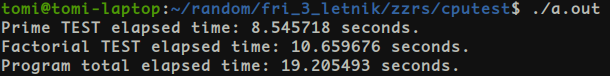
\includegraphics[scale=0.66]{Img/3_T_cputest.png}
	\caption{Časi izvajanja meritev na prenosnem računalniku s procesorjem Intel i5 7. generacije.}
	\label{fig:3_cputest1}
\end{figure}

\begin{figure}[H]
	\centering
	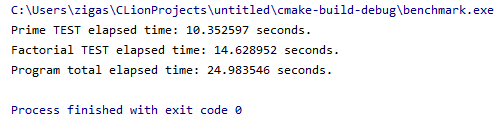
\includegraphics[scale=0.8]{Img/3_Z_cputest.png}
	\caption{Časi izvajanja meritev na osebnem računalniku s procesorjem Intel i5 3. generacije.}
	\label{fig:3_cputest2}
\end{figure}

\begin{figure}[H]
	\centering
	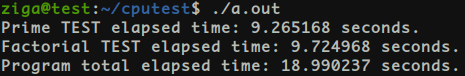
\includegraphics[scale=0.66]{Img/3_Azure_cputest.png}
	\caption{Časi izvajanja meritev na virtualnem računalniku na Azure platformi s procesorjem Intel Xeon Platinum 8. generacije.}
	\label{fig:3_cputest3}
\end{figure}

Rezultati meritev so precej zanimivi. Čeprav je procesor v prenosnem računalniku (i5 na sliki \ref{fig:3_cputest1}) 4 generacije novejši od procesorja v osebnem računalniku (i5 na sliki \ref{fig:3_cputest2}), je ta sodeč po meritvah na spletu 20\% počasnejši od procesorja v osebnem računalniku. Intuicija prav tako pravi, da lahko procesor v osebnem računalniku porablja več elektrike in bi zato moral biti hitrejši, čeprav je starejše generacije. V naših meritvah je procesor v prenosnem računalniku v vseh treh testih hitrejši od procesorja v osebnem. Razlogov za to je lahko več:

\begin{itemize}
	\item i5 7. ima kljub slabši splošni oceni boljšo oceno za eno jedro, kar je v teh dveh problemih relevantno;
	\item i5 7. generacije ima novejšo arhitekturo, ki ima določene optimizacije za ukaze, ki se uporabljajo v teh dveh problemih;
	\item čeprav lahko procesor v prenosnem računalniku vleče manj elektrike, pa se testa dovolj hitro končata, da je razlika v temperaturi, ki je posledica večjega toka elektrike, minimalna in lahko tudi prenosni procesor drži polno hitrost;
	\item razlika v predpomnilnikih obeh procesorjev;
	\item nekaj drugega;
\end{itemize}

Na to primerjavo se dobro nanaša tudi Xeon procesor (slika \ref{fig:3_cputest3}) na virtualnem računalniku, ki je zanimivo počasnejši v enem testu in hitrejši v drugem testu od prenosnega procesorja. Glede na to, da ima Xeon boljšo oceno za eno jedro kot prenosni procesor, bi moral biti hitrejši v obeh testih. Iz primerjav naših procesorjev in iz primerjav rezultatov na Azure platformi sklepamo, da je razlika posledica arhitekturnih razlik med procesorji ali pa razlik v pomnilniku. Xeon je namreč 48 jedrni procesor in mi si ga seveda delimo z ostalimi virtualkami, ki tečejo na tem procesorju, kar lahko vpliva na delovanje predpomnilnika.

\subsection{Test ob spremenjenih podatkovnih strukturah}

Rezultati tega testa bodo različni od zgornjih, ker smo zaradi izteka roka uporabe na platformi Azure morala zamenjati virtualni računalnik za drugega. Na tem drugem računalniku pa je lahko procesor drugačen in posledično se bodo tudi rezultati razlikovali.

V tem testu so tudi vse začetne številke preko katerih se preverja hitrost zmanjšane za faktor 10 (iz 10050000 na 1005000), saj bi drugače testiranje trajalo predolgo časa.

Z velikostjo podatkovnih struktur, ki jih procesor uporablja, se seveda spremeni tudi zmogljivost, kar smo izmerili v tem poglavju. Program, ki smo ga napisali za umetno breme na procesorju, smo spremenili tako, da je pognal teste ne samo z int in long, vendar tudi float in double. Čase izvajanja teh testov smo seveda tudi izmerili. Spet smo program pognali na svojih računalnikih, kot tudi na novi virtualki na Azure platformi. Rezultati meritev:

\begin{figure}[H]
	\centering
	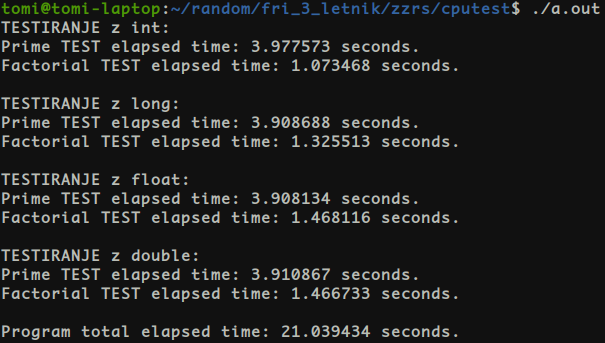
\includegraphics[scale=0.55]{Img/3_T_cputest2.png}
	\caption{Časi izvajanja meritev na prenosnem računalniku s procesorjem Intel i5 7. generacije.}
	\label{3_T_cputest1}
\end{figure}

\begin{figure}[H]
	\centering
	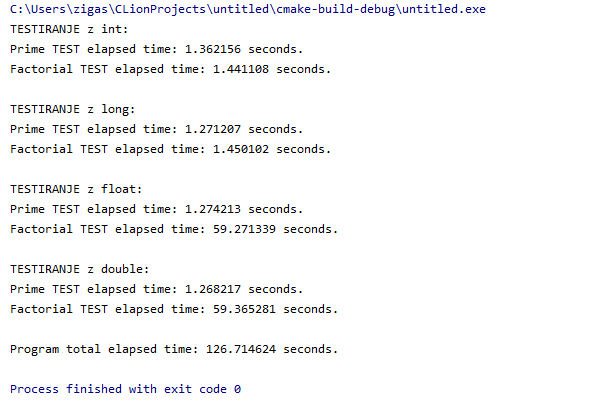
\includegraphics[scale=0.63]{Img/3_Z_cputest2.png}
	\caption{Časi izvajanja meritev na osebnem računalniku s procesorjem Intel i5 3. generacije.}
	\label{3_Z_cputest2}
\end{figure}

\begin{figure}[H]
	\centering
	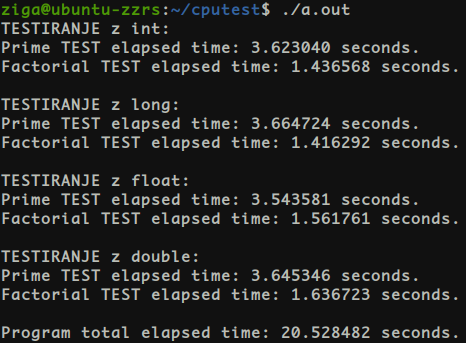
\includegraphics[scale=0.55]{Img/3_Azure_cputest2.png}
	\caption{Časi izvajanja meritev na virtualnem računalniku na Azure platformi s procesorjem Intel Xeon Platinum 8. generacije.}
	\label{Azure_cputest3}
\end{figure}

Rezultati tega testa so še bolj zanimivi kot prejšnji, saj nakazujejo, da je pravilna teorija o arhitekturnih razlikah. i5 3. generacije (slika \ref{3_Z_cputest2}) je namreč izredno počasen pri uporabi float in double, na kar predpomnilnik ne bi mogel tako močno vplivati.

Razlike med prenosnim i5 procesorjem (slika \ref{3_T_cputest1}) in Xeon procesorjem (slika \ref{Azure_cputest3}) v virtualnem računalniku pa je težje obrazložiti, saj smo morali ustvariti novo virtualko in razlike iz prejšnjega poglavja niso več konsistente z razlikami med prenosnim in strežniškim procesorjem v tem poglavju. Ni jasno ali je kriv predpomnilnik ali pa arhitektura, saj so razlike med posameznimi podatkovnimi strukturami še bolj zabrisane. Test za izračun praštevil z uporabo int je hitrejši na Xeonu, test za izračun faktoriele pa je hitrejši na prenosnem i5, čeprav se tudi tu uporablja int. Jasno pa je, da ima skupno rahlo prednost Xeon, ki je hitrejši za 1 sekundo, kar nakazuje na rahlo večjo zmogljivost.



\section{Zasedenost resursov}

Azure platforma ima tudi vgrajen način spremljanja zmogljivosti virtualnega računalnika. Na Azure portalu lahko namreč omogočimo funkcijo Insights, ki nam z 1-minutno natančnostjo spremlja in meri virtualko. Ker naš program traja le ~23.5 sekund, kar je očitno manj kot 1-minutna natančnost meritev in bi vplivalo na pomanjkljive rezultate funkcije Insights, smo morali na virtualnem računalniku pognati skripto, ki je program pognal 14-krat zaporedoma.

Insights ima kar nekaj dobrih lastnosti in funkcij, ena izmed njih je prikaz statističnih podatkov diagrama: v našem primeru smo prikazali povprečje in 95. percentil zasedenosti procesorja. Insights je seveda zasnovan za pregled delovanja na daljši rok, kot je običajni namen virtualnih računalnikov na Azure, zato so lastnosti kot sta dolgi rok hranjenja podatkov o zmogljivosti in statistični podatki o zmogljivosti veliko bolj pomembni kot natačnost, ki bi bila manjša kot 1 minuta. Na slikah \ref{3_kekw1} in \ref{3_kekw2} lahko vidimo uporabljene resurse.

Grafi, ki jih Insights izriše:

\begin{figure}[H]
	\centering
	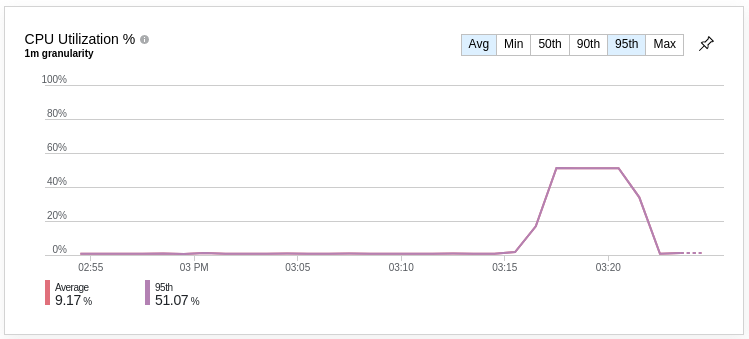
\includegraphics[scale=0.46]{Img/3_insights_cpu.png}
	\caption{Prikaz statistike rabe procesorja z uporabo funkcije Insights na Azure platformi.}
	\label{3_kekw1}
\end{figure}

\begin{figure}[H]
	\centering
	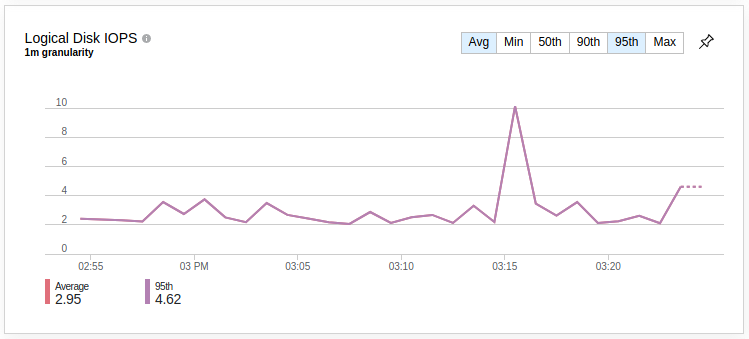
\includegraphics[scale=0.46]{Img/3_insights_iops.png}
	\caption{Prikaz statistike IO operacij na sekundo z funkcije Insights na Azure platformi.}
	\label{3_kekw2}
\end{figure}

\subsection{Zasedenost diskovnih in pomnilniških resursov}

Na platformi Azure imamo na voljo 1 disk z 30GB prostora. Naš program je napisan tako, da testira procesor in ne hitrost diskovnega pogona, kar lahko razberemo iz naslednjih slik \ref{3_kekw3} in \ref{3_kekw4}.


\begin{figure}[H]
	\centering
	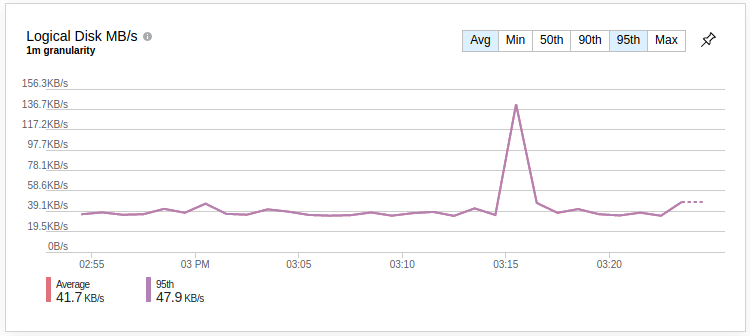
\includegraphics[scale=0.46]{Img/3_insights_iombs.png}
	\caption{Prikaz statistike prenosa podatkov na disk v MB na sekundo z uporabo funkcije Insights na Azure platformi.}
	\label{3_kekw3}
\end{figure}

\begin{figure}[H]
	\centering
	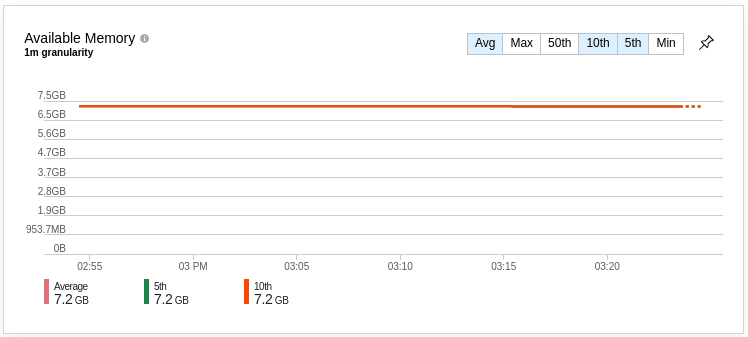
\includegraphics[scale=0.46]{Img/3_insights_mem.png}
	\caption{Prikaz statistike rabe pomnilnika z uporabo funkcije Insights na Azure platformi.}
	\label{3_kekw4}
\end{figure}

Grafi sledijo vsem pričakovanjem. V računalniku sta dve jedri, ker je program spisan za delovanje na enem jedru, je eno jedro popolnoma zasedeno, drugo pa skoraj prazno. To v statistikah pomeni zasedenost 50\%. Ob zagonu skripte za izvajanje programa, se mora program naložiti v pomnilnik, kar pomeni skok v rabi diska. Naslednje iteracije imajo program že v pomnilniku, ki pa se praktično ne spremeni, saj je program zelo majhen in uporablja zelo malo pomnilnika.

Celotno trajanje vseh 14 izvedb je bilo 330 sekund, povprečje pa je bilo 23.6 sekund, kar je precej drugače od prejšnjega testa. Razloga za to sta po naših mnenjih dva:
\begin{itemize}
	\item daljše trajanje zasedenosti procesorja pomeni da procesor ne more teči z višjo uro toliko časa, kot lahko pri eni sami izvedbi, saj bi se lahko pregrel;
	\item med vsemi 14 izvajanji programa smo opazili tudi nekaj izvajanj, ki so odstopali od tega povprečja trajanja, torej je možno, da smo pri prejšnjem testu ravno naleteli na izvedbo, ki je bila precej pod povprečnim časom trajanja;
\end{itemize}
Pravi odgovor je verjetno kombinacija teh dveh razlogov.

Ostalih diagramov, ki jih insights prikaže nidmo dodali v poročilo, saj so rezultati pričakovani in ni posebnih zanimivosti na diagramih. Vsi pa imajo natančnost 1 minute.




\subsection{Obremenitev pomnilnika}

V tem razdelku bomo zapolnili pomnilnik na 90\% in nato izvajali program testiranja CPU in program, ki bo zapolnil pomnilnik še za 10\%.
Ukaz za zapolnitev pomnilnika na 90\% smo našli na stackexchange.com \cite{mem90Fill} in sproži program stress-ng.
\begin{verbatim}
stress-ng --vm-bytes $(awk '/MemAvailable/{printf "%d\n", $2 * 0.9;}
' < /proc/meminfo)k --vm-keep -m 1
\end{verbatim}
Ta ukaz zagotovi da operacijski sistem ne bo uporabljal tega dela pomnilnika in da ga ne bo zamenjal z drugimi segmenti z diska. Pomankljivost tega ukaza je, da uporablja celotno jedro procesorja za svoje izvajanje. Zaradi tega, ko smo poganjali naš program, ki testira CPU se je njegovo izvajanje povečalo iz 22 sekund na 30 sekund. Mislimo, da se je to zgodilo zaradi dodatnih programov, ki so delovali na jedru na katerem se je izvajal naš program, ker je bilo drugo jedro popolno zasedeno zaradi ukaza stress-ng. Na spodnjih slikah \ref{fig:3_ram1} in \ref{fig:3_ram2} lahko vidite pomnilnik alociran z ukazom stress-ng in uporabo diska pri menjavah pomnilnika. 


\begin{figure}[H]
	\centering
	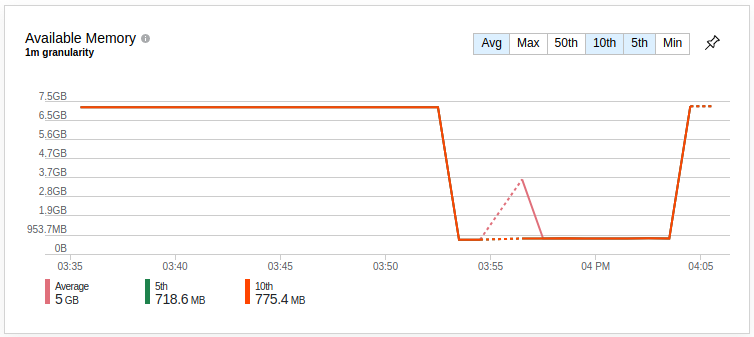
\includegraphics[scale=0.46]{Img/3_ram_obr1.png}
	\caption{Prikaz pomnilnika, ki je na voljo z uporabo funkcije Insights na Azure platformi.}
	\label{fig:3_ram1}
\end{figure}

Na sliki \ref{fig:3_ram1} lahko vidimo, da z zapolnitvijo pomnilnika, mora operacijski sistem uporabiti disk za shranjevanje podatkov. To je razvidno iz črtkane črtice, ki narašča in nato hitro pade. Istočasno je bila zajeta tudi slika \ref{fig:3_ram2} na kateri se vidi trenutek, ko je operacijski sistem uporabljal disk, ko mu je primanjkovalo rama. 

\begin{figure}[H]
	\centering
	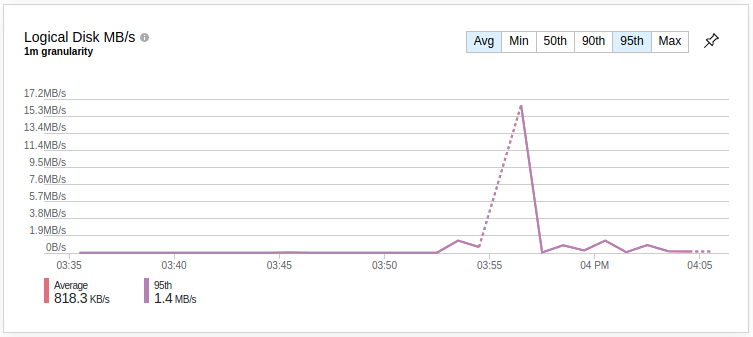
\includegraphics[scale=0.46]{Img/3_ram_obr2.png}
	\caption{Prikaz  uporabe diskovja z uporabo funkcije Insights na Azure platformi.}
	\label{fig:3_ram2}
\end{figure}


Naš program smo zagnali 14x zaporedoma (da se lahko vidi na grafih Azure platforme, ker je interval na 1 minuto), medtem, ko je bilo 90\% pomnilnika zasedenega. Celotni virtualni računalnik je med izvajanjem postal zelo neodziven (npr. rabil je v povprečju 4 sekunde več pri vzpostavitvi ssh povezave in tudi izvajanje programov postane bolj neodzivno). Prav izvajanju  tako je pri izvajanju 5. instance programa, ko je pomnilnik prišel do 100\%, Operacijski sistem ubil vse naše procese, da je sprostil svoje resource. To lahko tudi razberemo iz slik \ref{fig:3_ram3} in \ref{fig:3_ram4}.


\begin{figure}[H]
	\centering
	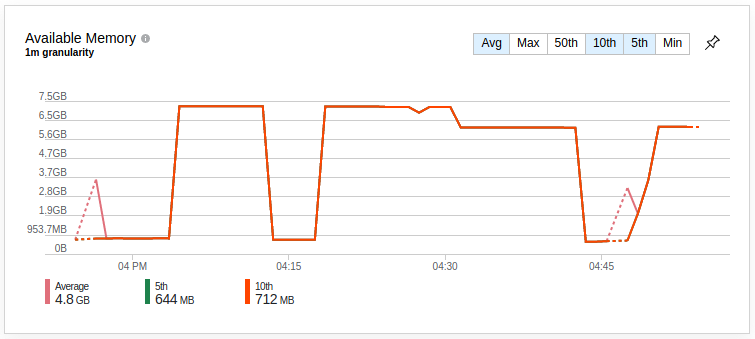
\includegraphics[scale=0.46]{Img/3_ram3.png}
	\caption{Prikaz pomnilnika, ki je na voljo z uporabo funkcije Insights na Azure platformi.}
	\label{fig:3_ram3}
\end{figure}

\begin{figure}[H]
	\centering
	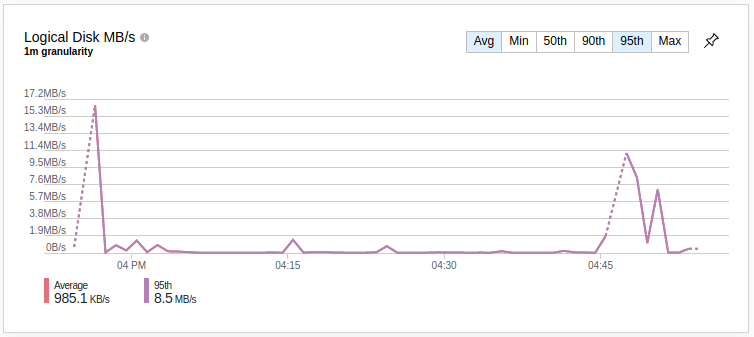
\includegraphics[scale=0.46]{Img/3_ram4.png}
	\caption{Prikaz  uporabe diskovja z uporabo funkcije Insights na Azure platformi.}
	\label{fig:3_ram4}
\end{figure}


Po testiranju CPU z našim programom smo napisala program, ki statično alocira pomnilnik. V programu smo izklopili menjavo alociranih delov pomnilnika. Če smo preseglai pomnilnik, ki je bil na voljo, je operacijski sistem ubil program. Vendar se na grafih Azura ne pokaže nič, saj je interval časa po katerih se riše graf prevelik.

\subsection{Test zmogljivosti baze MySQL}

Za zadnji test zmogljivost smo izvedli preprost test baze MySQL. Napisali smo preprost program, ki najprej vzpostavi povezavo z bazo, nato v njo 500-krat zaporedoma vstavi in odstrani vrstico. Sama polja, ki jih vstavlja v tabelo v bazi sicer niso pomembna, lahko pa omenimo da vstavljamo 3 nize znakov in eno celo število. Izmerili smo čas pred začetkom vstavljanja in brisanja, ter čas po vseh 500 izvedbah. Nato smo razliko teh dveh časov delili s številom vseh ponovitev, torej 500, da smo dobili povprečen čas trajanja 1 ponovitve vstavljanja in brisanja iz baze.

Poleg samega programa za testiranje, smo ustvarili tudi skripto, ki je le ta program pognala vzporedno v nekem številu. Npr.: vzporedno smo pognali 50 kopij tega programa in merili čas izvajanja v vsaki kopiji posebej. Rezultati teh testiranj so spodaj.

\begin{table}[H]
	\centering
	\begin{tabular}{ | r | r | r | r | }
		\hline
		Število kopij programa & Povprečni čas vstavitve in brisanja [ms]  \\
		\hline
		1 & 13.5 \\
		5 & 25.2 \\
		10 & 28.2 \\
		25 & 29.2 \\
		50 & 34.7 \\
		75 & 39.9 \\
		150 & 61.3 \\
		\hline
	\end{tabular}
	\caption{Povprečni čas izvajanja 1 vstavitve in brisanja pri določenem številu kopij programa.}
	\label{table:1_chunks}
\end{table}

Kot pričakovano se čas 1 vstavitve in brisanja slabša, vendar morda ne zaradi pričakovanega razloga. V tej virtualki sta na voljo le 2 jedri, kar pomeni, da se dejansko lahko izvajata le 2 procesa hkrati. Sklepamo, da je daljši čas ni posledica paralelnega izvajanja večih kopij programa, vendar je le ta posledica odločanja operacijskega sistema, kateri proces dobi procesorski čas. Operacijski sistem vsaki kopiji programa dodeli nekaj časa izvajanja, potem pa ga odvzame in da naslednjemu procesu. Nikoli ne pride do dejanskih težav pri dohajanju podatkovne baze z zahtevami, ki nanjo pridejo, saj bi se to poznalo kot hud porast v času izvajanja, ki pa ga v tabeli ne zasledimo. Je pa res, da se pri zadnji meritvi s 150 kopijami programa, čas močno poslabša, vendar ne dovolj za kakšne večje sklepe. 150 je namreč tudi maksimalno število hkratnih povezav, torej je to nekakšen najslabši primer za bazo.

Predvidevamo, da bi bilo za kakšen bolj realen test podatkovne bazo potrebno vzpostaviti nek porazdeljen test, ki bi iz večih lokacij izvajal bolj kompleksne zahteve na bazo, dokler ta ne bi prišla do mej uporabnosti.

\section{Zaključek}
Na trgu je veliko orodij za testiranje Oblačnih platform, nekatera so, kot smo ugotovili plačljiva, spet druga so brezplačna velika večina plačljivih orodij nima veliko izboljšav izmed najboljših brezplačnih orodij. To smo lahko videli pri testiranju oblačne platforme Azure, kjer smo uporabljali brezplačna orodja in še zmeraj dobili zadovoljive rezultate. Pri ročnem testiranju Azure se nam zdi iz naših ugotovitev, da se lahko še največ naučimo prav iz njih, saj lahko z ročnim pisanjem kode testiramo veliko stvari, ki jih orodja narejena zato ne morejo, ker so nekatere stvari preveč specifične uporabnikovim zahtevam. Testiranje platforme Azure je pokazalo njeno slabosti in prednosti, pod šibkosti bi lahko vmestili lokacijo računalnika, med prednosti pa njeno odlično računsko moč. Vse to je seveda predpostavljeno z dejstvom, da smo uporabljali zastonjski račun na platformi, ki ima dokaj omejen nabor funkcionalnosti in strojne opreme.

